\section{Support Vector Regression (SVR)}

\mode<presentation>{
\begin{frame} 
    \begin{center} \huge
        \secname
    \end{center}
    \begin{center}
    SVMs for regression problems   
    \end{center}
\end{frame}
}

\begin{frame}\frametitle{The regression setting}

\mode<article>{
\underline{The regression setting}:
}

\begin{itemize}
\item[] \underline{Data}:\\

    \item[]$
    \big\{ \big(\vec x^{(\alpha)}, y_{T}^{(\alpha)}\big)\big\}_{\alpha=1}^{p}
    $ with $\vec x \in \R^{N}$ and $y_{T} \in \R${}

\item[] \underline{Model}:\\
    linear neuron: $
        y(\vec x; \vec w, b) = \vec w^{\top} \vec x + b$
        
\item[] \underline{Objective}:\\
    \begin{itemize}
    \item ERM: $\min_{\vec w,b} E^{T}$
    \item SRM: $\min_{\vec w,b} \frac{1}{2} \lVert \vec w \rVert + C R_{\text{emp}}(\vec w,b)$
    \end{itemize}

    
\end{itemize}


\begin{figure}[h]
     \centering
     \savebox{\imagebox}{
	 \includegraphics[width=0.35\textwidth]{img/regression_1d_linear}}%
     \begin{subfigure}[t]{0.35\textwidth}
         \centering
         \usebox{\imagebox}% Place largest image
         \caption{linear regression}
         \label{fig:regression1dlinear}
     \end{subfigure}
     \hspace{10mm}
     \begin{subfigure}[t]{0.35\textwidth}
         \centering
         \raisebox{\dimexpr.5\ht\imagebox-.5\height}{% Raise smaller image into place
         \includegraphics[width=0.99\textwidth]{img/regression_1d_nonlinear}
         }
         \caption{non-linear regression}
         \label{fig:regression1dnonlinear}
     \end{subfigure}
     \caption{scalar regression with 1D input}
	 \label{fig:regression}
\end{figure}



\end{frame}

\subsection{The $\varepsilon$-insensitive cost function for regression}

\begin{frame}\frametitle{\subsecname}

\slidesonly{\vspace{-5mm}}

\begin{equation}
e(y(\vec x; \vec w, b), y_{T}; \varepsilon)
= e(\underbrace{y(\vec x)}_{\mathclap{\text{for brevity}}}, y_{T}; \varepsilon)
= \max(~0~, \big|y(\vec x) - y_{T}\big|-\varepsilon~)
\end{equation}

\begin{itemize}
\item The cost function is parameterized by $\varepsilon$ that is chosen a priori.
\notesonly{\item[$\leadsto$] no error for $
y(\vec x) \in \lbrack y_{T}-\varepsilon, y_{T}+\varepsilon\rbrack$
otherwise,
\item[$\leadsto$] linear error
}
\end{itemize}

\slidesonly{\vspace{-2mm}}

\begin{figure}[h]
     \centering
	 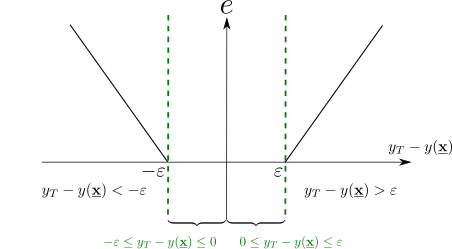
\includegraphics[width=0.6\textwidth]{img/cost_eps}%
	 \mode<article>{
     \caption{The cost function}
     }
	 \label{fig:cost}
\end{figure}

The SRM objective becomes:

\slidesonly{\vspace{-5mm}}

\begin{equation}
    \min_{\vec w,b} \frac{1}{2} \lVert \vec w \rVert + C R^{\varepsilon}_{\text{emp}}(\vec w,b)
    \slidesonly{
    \quad
    \text{using}\quad R^{\varepsilon}_{\text{emp}}(\vec w,b) = \frac{1}{p}\sum_{\alpha=1}^{p} e(y(\vec x), y_{T}; \varepsilon)
     %\max(0, \big|y(\vec x) - y_{T}\big|-\varepsilon)
     }
    \label{eq:srmeps}
\end{equation}

\notesonly{
using 
\begin{align}
    R^{\varepsilon}_{\text{emp}}(\vec w,b) &= \frac{1}{p}\sum_{\alpha=1}^{p} e(y(\vec x), y_{T}; \varepsilon)\\
    &= 
    \frac{1}{p}\sum_{\alpha=1}^{p} \max(0, \big|y(\vec x) - y_{T}\big|-\varepsilon)
    \label{eq:srmepscost}
\end{align}
}
    
\end{frame}

\subsection{Deriving the primal problem for $\varepsilon$-SVR}

\begin{frame}{Only}\frametitle{\subsubsecname}

\begin{figure}[h]
     \centering
	 \includegraphics[width=0.45\textwidth]{img/regression_1d_linear_margin}%
     \caption{Linear model (no points outside the margin)}
	 \label{fig:model_margin}
\end{figure}

\slidesonly{\vspace{-5mm}}

\begin{itemize}
\item[(i)]
Simplify assumptions (will be relaxed later)\notesonly{\footnote{This is based on my understanding of Ch. 9 from \citep{scholkopf2001learning}.}}

\begin{enumerate}
    \item<only@1-> perfect regression solution, i.e. zero error $\varepsilon$-insensitive cost,
    \item<only@2,3> the constrained regression problem\\
		\only<2>{
        \begin{equation}
        \begin{array}{ll}
        \min_{\vec w, b} & \frac{1}{2} \lVert \vec w \rVert_{2}^{2}\\
        \text{subject to} & 
        y(\vec x^{(\alpha)}) - y_{T}^{(\alpha)} \le \varepsilon\\
        &
        y_{T}^{(\alpha)} - y(\vec x^{(\alpha)}) \le \varepsilon \quad \text{for }\alpha=1,\ldots,p
        \end{array}
        \end{equation}  
        }
        \only<3>{
        Substituting $y(\vec x^{(\alpha)}) = \vec w^{\top} \vec x^{(\alpha)} + b$ yields:\\

        \begin{equation}
        \begin{array}{ll}
        \min_{\vec w, b} & \frac{1}{2} \lVert \vec w \rVert_{2}^{2}\\
        \text{subject to} & 
        \vec w^{\top} \vec x^{(\alpha)} + b - y_{T}^{(\alpha)} \le \varepsilon\\
        &
        y_{T}^{(\alpha)} - \vec w^{\top} \vec x^{(\alpha)} - b \le \varepsilon \quad \text{for }\alpha=1,\ldots,p
        \end{array}
        \end{equation}  
        }
\end{enumerate}
\end{itemize}
    
\end{frame}

\newpage

\begin{frame}{Only}\frametitle{\subsubsecname}

\slidesonly{\vspace{-3mm}}

\begin{figure}[h]
     \centering
     \savebox{\imagebox}{
	 \includegraphics[width=0.35\textwidth]{img/regression_1d_linear_margin_phi}}%
     \begin{subfigure}[t]{0.35\textwidth}
         \centering
         \usebox{\imagebox}% Place largest image
         \mode<article>{
         \caption{}
         }
         \label{fig:violate_within_margin}
     \end{subfigure}
     %\hspace{2mm}
     \begin{subfigure}[t]{0.35\textwidth}
         \centering
         \raisebox{\dimexpr.5\ht\imagebox-.5\height}{% Raise smaller image into place
         \includegraphics[width=0.99\textwidth]{img/cost_eps_phi}
         }
         \mode<article>{
         \caption{}
         }
     \end{subfigure}
     \mode<article>{
     \caption{Relaxed assumptions}
	 }
	 \label{fig:relaxed}
\end{figure}

\slidesonly{\vspace{-5mm}}

\begin{itemize}
\item[(ii)]
Relax constraints by allowing for errors\\

\only<1>{
\question{Why would we ever want to allow for errors?}\\
}

\notesonly{
- in order to reduce overfitting to noise or outliers in the training data.
}

\only<2->{
\begin{enumerate}
    \item<only@1-> possibly more robust to noise and outliers,
    \item<only@2-> constrained regression problem\notesonly{ that allows for errors} (with slack variables $\varphi_\alpha$)\\
    
\slidesonly{\vspace{-3mm}}

		\only<2->{
        \begin{equation}
        \begin{array}{ll}
        \min_{\vec w, b\only<3>{,\{\varphi_\alpha, \varphi_\alpha^*\}}} & \frac{1}{2} \lVert \vec w \rVert_{2}^{2} \only<3->{+ C \frac{1}{p} \sum_{\alpha}^p (\varphi_\alpha + \varphi_\alpha^*)}\\
        \text{subject to} & 
        \vec w^{\top} \vec x^{(\alpha)} + b - y_{T}^{(\alpha)} \le \varepsilon + \varphi_\alpha\\
        &
        y_{T}^{(\alpha)} - \vec w^{\top} \vec x^{(\alpha)} - b \le \varepsilon + \varphi_\alpha^*\\
        & \varphi_\alpha, \varphi_\alpha^* \ge 0 \qquad\qquad\qquad\slidesonly{\qquad\qquad} \text{for } \alpha=1,\ldots,p
        \end{array}
        \label{eq:primaleps}
        \end{equation}
        
        \only<3->{with $C>0$ ($C$ penalizes model error)}
        }
        
        \only<2>{
        \question{How do we prevent solutions with arbitrarily large $\varphi_\alpha, \varphi_\alpha^*$ that prevent any violation of the constraints?}\\
        
        \notesonly{
        - The second term in the minimization objective that is parameterized by $C$ takes care of this, as it penalizes model error.\\
        
        \eqref{eq:primaleps} gives us the \emph{primal problem} for $\varepsilon$-SVR.
        }
        }
        
        \only<4>{\question{Should we divide the sum by 2 since we're adding $(\varphi_\alpha + \varphi_\alpha^*)$ inside the sum?}}
        
        
        \notesonly{
        - No, this is not necessary. $\varphi_\alpha$ and $\varphi_\alpha^*$ describe error on opposite sides of the line we are fitting. A point cannot fall below \textbf{and} above a line at the same time. One of the slack variables for any point will always be zero.
        
        At this point we can define the empirical risk term $R^{\varepsilon}_{\text{emp}}$ in \eqref{eq:srmeps} in terms of the slack variables:
        
        }
        \only<5>{

\slidesonly{\vspace{-5mm}}
\slidesonly{
\begingroup
\footnotesize
}
        \begin{equation}
        \min_{\vec w,b} \frac{1}{2} \lVert \vec w \rVert^2_2 + C \; \overbrace{\frac{1}{p} \sum_{\alpha=1}^p (\varphi_\alpha + \varphi_\alpha^*)}^{=:R^{\varepsilon}_{\text{emp}}(\vec w,b)}
    \end{equation}
\slidesonly{
\endgroup
}
        }
        
\end{enumerate}
}
\end{itemize}
    
\end{frame}

\begin{frame}\frametitle{Making predictions using $\varepsilon$-SVR}


\slidesonly{\vspace{-5mm}}

\begin{figure}[h]
     \centering
     \savebox{\imagebox}{
	 \includegraphics[width=0.45\textwidth]{img/regression_1d_linear_margin_phi}}%
     \begin{subfigure}[t]{0.4\textwidth}
         \centering
         \usebox{\imagebox}% Place largest image
         \caption{linear regression}
     \end{subfigure}
     \hspace{5mm}
     \visible<2>{
     \begin{subfigure}[t]{0.4\textwidth}
         \centering
         \raisebox{\dimexpr.5\ht\imagebox-.5\height}{% Raise smaller image into place
         \includegraphics[width=0.88\textwidth]{img/regression_1d_nonlinear_margin_phi}
         }
         \caption{non-linear regression}
         \label{fig:regression1dnonlinear}
     \end{subfigure}
     }
     \mode<article>{
     \caption{SVR for linear and non-linear regression}
     }
	 \label{fig:svrregression}
\end{figure}


\slidesonly{\vspace{-5mm}}

\begin{equation}
\vec w^* = \sum_{\alpha=1}^p (\lambda_\alpha - \lambda_\alpha^*) \vec x^{(\alpha)} \stackrel{\substack{\text{either}\\ \lambda_\alpha \text{ or } \lambda_\alpha^* \ne 0\\\text{for SVs}}}{=} \sum_{\beta\in\mathrm{SV}} (\lambda_\beta - \lambda_\beta^*) \vec x^{(\beta)}
\end{equation}

\begin{equation}
y(\vec x) = b^* + \sum_{\beta\in\mathrm{SV}} (\lambda_\beta - \lambda_\beta^*) 
\only<2>{
\underbrace
}
{
\big( \vec x^{(\beta)} \big)^\top \vec x
}
\only<2>{
_{\text{kernels!}}
}
\end{equation}

\end{frame}

